
\textbf{Локализация}. Принципиально противоположным термализации будет локализация. Так бывает, что система сохраняет информацию о начальных условиях даже при $t \to \infty$ (fig. \ref{fig:BASE}, \blue{blue curve}) и $A = A(\psi_0)$.  Например мы можем разделить систему на две равные подсистемы $\Omega_1,\, \Omega_2$, заселить только $\Omega_1$ и следить за контрастностью
\begin{equation*}
	\mathcal{I} = \frac{N_{\Omega_1}-N_{\Omega_2}}{N_{\Omega_1}+N_{\Omega_2}}.
\end{equation*}
Так в \cite{schreiber_observation_2015} в 1D в качестве $\Omega_1$ выбрали чётные узлы решётки (fig. \ref{fig:loc1}), а в \cite{Choi_2016} в 2D за $\Omega_1$ взяли левую часть системы (fig. \ref{fig:loc2D1}). Как раз для $\mathcal{I}(t)$ уже видно заявленное термальное поведение, когда $\mathcal{I}(t \gg \tth) \approx 0$, но в какой-то момент случается переход к локализации и $\mathcal{I} (t \gg \tth) \approx \const > 0$. Такое поведение характерно при добавление в систему frozen noise $\Delta > 0$, первые данный эффект был описан by Anderson \cite{PhysRev.109.1492}.

Для одночастичной задачи было бы логичным предположить, что такое поведение возникает из-за локализации собственных функций. Действительно, в fig. \ref{fig:loc1} представлены собственные состояния гамильтониана при разных уровнях шума.  

% Здесь хотелось бы добавить немного конкретики, в этом эссе будет рассматриваться Hubbard model (которая иногда сводится к Heisenberg model, см. приложение):



\begin{figure}[h]
    \centering
    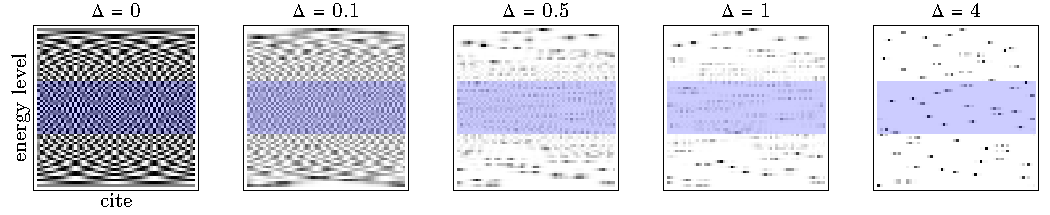
\includegraphics{imgs/evecs.pdf}
    \caption{Eigenvectors for $L=60$ and $N=1$}
    \label{fig:loc1}
\end{figure}

